\chapter{Priama a nepriama úmernosť, percentá, pomer}

\begin{example}
	Do každého pecňa chleba pridávajú v miestnej pekárni slnečnicové, ľanové, konopné a tekvicové semienka v pomere 5:3:4:2. Koľko kilogramov slnečnicových semienok treba ešte pridať, ak ľanové, konopné a tekvicové semienka majú spolu hmotnosť 6,3 kg?
\end{example}

\begin{example}
	Alica kúpila zmes orechov obsahujúcich kešu orechy, lieskové orechy a arašidy zastúpené v pomere 1:2:3. Vypočítajte v gramoch hmotnosť celej zmesi, ak arašidy majú hmotnosť 90 gramov.
\end{example}

\begin{example}
	Osobný automobil prešiel trasu z Trenčína do Ružomberka za 1 hodinu a 48 minút. Tieto dve mestá sú od seba vzdialené 144 kilometrov. O koľko minút by si vodič skrátil cestu, ak by na nej išiel rýchlosťou 90 kilometrov za hodinu?
\end{example}

\begin{example}
	Brigádnici Ivan, Lea a Dana zarobili spolu 480 eur. Ivan zarobil tretimu z týchto peňazí. Zvyšné peniaze zarobili Lea a Dana v pomere 3:1. Koľko eur zarobila Lea?
\end{example}


\begin{example}
	Skupina troch dievčat vyhrala v prírodovednej súťaži 30 eur. Kamila, Magda a Zuzka si výhru rozdelili podľa výkonu v pomere 3:4:5. Ktorá z možností je nesprávna?
	
	\begin{enumerate}
		\item Kamila a Magda majú spolu viac eur ako Zuzka.
		\item Zuzka a Kamila majú spolu 20 eur.
		\item Magda a Zuzka majú spolu o 16 eur viac ako Kamila.
		\item Kamila má o 5 eur menej ako Zuzka.
	\end{enumerate}
\end{example}

\begin{example}
	Vlasta, Klára a Zuzana si rozdelili odmenu v pomere 5:8:12. Sestry Zuzana a Klára dostali spolu 120 eur. Koľko eur dostala Vlasta?
\end{example}

\begin{example}
	Priemerná spotreba automobilu je 5,6 litra na 100 kilometrov. Koľko litrov paliva sa pri priemernej spotrebe minulo, ak automobil prešiel 800 kilometrov? Výsledok uveď s presnosťou na 2 desatinné miesta.
\end{example}

\begin{example}
	Reštaurácia bola v čase obeda plne obsadená. Kým v reštaurácii obsluhovali len traja časnící, hostia čakali na obedové menu v priemere 45 minút. Koľko minút budú v priemere hostia čakať, ak sa k trom obsluhujúcim čašníkom pridajú ďalší dvaja časnící obsluhujúci rovnako rýchlo.
\end{example}

\begin{example}
	Po zdražení o 40\% stál zápisník 10,50 eur. Koľko eur by stál zápisník, keby namiesto 40\%-ného zdraženia zdražel len o 20\%?
\end{example}

\begin{example}
	Jana, Alena a Karol spolu nazbierali 40\% hmotnosti papiera z celej triedy. Jana nazbierala 93 kilogramov, Alena nazbierala 81 kilogramov a Karol nazbieral 96 kilkogramov. Koľko kilogramov nazbierala celá trieda?  
\end{example}

\begin{example}
	V predajni mobilného operátora mali týždeň zliav. Mobilné telefón LF 34 zľacnel zo 769 eur na 544 eur. Približne o koľko precent zľacnel tento mobilný telefón?
\end{example}

\begin{example}
	10 gramov kivi obsahuje rovnaké množstvo vitamínu C ako 50 gramov pomarančov. 100 gramov šípok obsahuje rovnaké množstvo vitamínu C ako 200 gramov kivi. Koľko gramov pomarančov obsahuje rovanké množstvo vitamínu C ako 50 gramov šípok?
\end{example}

\begin{example}
	V recepte na lečo sa odporúča zamiešať paradajky, papriku a cibuľu v pomere 4:3:1. Pani kuchárka už pripravila cibuľu aj papriku, pričom cibule bolo 5 kg menej ako papriky. Koľko kg paradajok bude potrebovať podľa tohoto receptu?
\end{example}

\begin{example}
	Karol si šetril na tablet. Keď mal ušetrených 178 eur zistil, že cenu tabletu znížili o 25\%, takže si ho môže hneď kúpiť a ešte mu zostane z ušetrených peňazí 13 eur. Koľko eur stál tablet pre zľacnením?
\end{example}

\begin{example}
	Na tácke boli marhuľové a slivkové koláče v pomere 3:2. Po zjedení troch marhuľových koláčov je šanca vybratia marhuľového alebo slivkového koláča rovnaká. Koľko koláčov bolo na začiatku na tácke?
\end{example}

\begin{example}
	Novákovci plánuju v priebehu septembra opraviť fasádu domu. S prácami sa začne 2. septembra. Počas nedieľ a sviatkov sa pracovať nebude. Tieto dni sú v kalendári podčiarknuté. 
	
	\begin{center}
		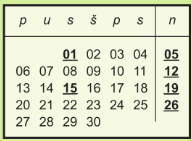
\includegraphics{assets/kalendar.png}
	\end{center}
	Štyria robotníci by opravili fasádu za 10 dní. Kedy možno očakávať skončenie prác, ak budú pracovať len 2 robotnící? Prepokladáme, že všetci robotnící pracujú rovnako výkonne. 
\end{example}